\documentclass[12pt]{article}

\usepackage{amsmath,amsfonts}
\usepackage{todonotes}
\usepackage{hyperref}
\usepackage{url}
\usepackage{graphicx}
\usepackage{algpseudocode}
\usepackage{algorithm}

\newcommand{\parex}{\texttt ParEx}
\newcommand\norm[1]{\left\lVert#1\right\rVert}
\newcommand{\Real}{\mathbb{R}}
\newcommand{\spar}{s_\textup{seq}}


\begin{document}

\title{A Suite of Parallel Extrapolation Solvers for Initial Value Problems}
\author{David I. Ketcheson
\thanks{King Abdullah University of Science and Technology}
Humam Alwassel
\thanks{Cornell University} \and
Marc Cayuela Rafols
\thanks{Polytechnic University of Catalonia} \and
}

\maketitle

\begin{abstract}
We present \parex, an implementation of extrapolation 
methods for solving initial-value ordinary differential equations
in parallel, written in Python.
%Extrapolation methods naturally 
%admit an efficient parallel implementation that can take advantage
%of multiple  processors.  
The implementation includes both explicit and  linearly-implicit methods, with
adaptive step size and order control as well as dense output.
We show that the 
explicit methods outperform widely-used explicit solvers for a 
range of test problems.
%as long as the derivative evaluation is moderately expensive.  
The linearly implicit solvers are competitive with existing solvers
for stiff problems.%, and examples show that they can be made 
%more efficient through further work on the algebraic solver
%subroutines.
The solvers are
implemented in pure Python and are thus highly portable and 
relatively easy to understand.
A test suite is included with the package.
\end{abstract}


%\keywords{extrapolation, initial value problem, parallel algorithms}


\section{Introduction}
Although the idea of extrapolation goes back to Richardson's
1910 paper \cite{richardson1910approximate},
its application to the solution of initial value problems
was not explored until the 1960's, most notably by Gragg \cite{gragg1965extrapolation}.
The idea was pursued enthusiastically over the next three
decades, and a number of general-purpose extrapolation codes
were developed, including ODEX \cite{HairerODEX}, EULSIM, and several related codes \cite{extrapolation_codes}.  
Eventually some of these codes included 
all the standard features of production ODE solvers:
error control, order and step-size adaptation, and 
efficient dense output.
However, comparisons of extrapolation methods with
the best Runge--Kutta and multistep methods showed 
extrapolation to be somewhat less efficient \cite{Shampine1986,hosea1994a}.
Subsequently, work on extrapolation methods subsided.

Each step of an extrapolation solver consists
of many independent -- and therefore potentially concurrent --
stages.  This was clear to their early developers 
(see e.g. \cite{Deuflhard1985}) but was never exploited
in implementations.  Possible reasons for this are
the long prevalence of single-processor computers
and the efficient use of parallelism ``across the system''
(e.g. via domain decomposition) for large systems of ODEs.
Although a few works (such as \cite{Korch2011}) have briefly explored the performance of
parallel extrapolation in a limited setting, no
implementation is available.

Most modern desktop computers contain enough
processors to take full advantage of the concurrency offered by extrapolation.
On supercomputers, domain decomposition is often insufficient
to fully exploit the large numbers of processors available.  Furthermore, domain decomposition
requires synchronization at each stage, whereas the concurrency
available in extrapolation methods requires synchronization
only once per step.  Thus extrapolation and similar methods
can be seen as a communication-avoiding alternative (or supplement)
to traditional domain decomposition.  Reducing synchronization
is essential to achieving high performance on current- and
next-generation supercomputers \cite{rude2016research}.
Thus conditions seem ripe for 
renewed investigation of parallel extrapolation methods.
Recently it was shown that with the added
advantage of concurrency, explicit extrapolation methods 
are theoretically more
efficient high-order Runge--Kutta methods \cite{2014_hork}.
In addition, a simple parallelization of the ODEX code
was shown to give promising results, even without
order adaptivity.

In this article, we present fully adaptive parallel
solvers based on extrapolation of low-order
methods.  Both explicit methods (for non-stiff problems)
and linearly implicit methods (for stiff problems) are included.
Most of the algorithmic details are based on
the theoretical and practical developments
in this area during the 80's and 90's, which are
summarized well in \cite{hairer1993,Hairer:ODEs2}.
Some different algorithmic choices are made to better
take advantage of concurrency;
those are highlighted in this article.

The solvers are implemented in Python.  Python is
a high-level language designed to be very readable,
but its performance is similar to that of MATLAB, and not as good as compiled languagues
like C and Fortran.
Nevertheless, we chose Python
as the language of implementation for the following
reasons:
\begin{itemize}
	\item For large systems, the performance bottleneck 
    		in an explicit ODE solver
    		is evaluation of the right-hand-side function $f$.
            This can be implemented in Fortran or C and 
            called from Python using simple automated tools.
	\item Similarly, for linearly implicit solvers the performance
    		bottlenecks are evaluation of the  jacobian of 
            $f$ and solution of linear algebraic systems.
            These can be implemented in a low-level language
            and called from Python.
     \item Python code is exceptionally easy to read and understand.
     		It is usually much shorter than equivalent C code,
            for instance.
     \item Python code is highly portable, since it is included
     		on all Unix-based systems and requires no compilation.
     \item Unlike proprietary languages such as MATLAB or
     		Mathematica, Python
     		is free and depends only on lower-level libraries 
            (such as those for linear algebra) that are fully
            open-source.
\end{itemize}

Following up on the theoretical analysis and proof-of-concept
presented in \cite{2014_hork}, we
show that explicit parallel extrapolation is competitive
with or superior to existing highly-optimized
state-of-the-art solvers for non-stiff problems.

Implementation of a solver for stiff problems is substantially
more complex, since it typically involves solvers for
linear and nonlinear algebraic systems, which bring a
host of potential algorithmic choices and tradeoffs, many
of which are problem-dependent.  Since our parallel
semi-implicit extrapolation solvers are the first of their
kind, we do not expect them to outperform contemporary
stiff solvers that have undergone generations of optimization.
Nevertheless, we show that for a range of test problems
the new solvers are highly efficient in terms of the number
of sequential linear solves required.  It seems likely
that further development on the algebraic solver side may
make these methods more efficient than their Runge--Kutta
and multistep counterparts.

\section{Background}
We are concerned with one-step methods for the solution of the initial value ODE
\begin{align} \label{ivp}
y'(t) & = f(y) & y(t_0) = y_0,
\end{align}
where $y\in\Real^m$, $f: \Real^m \to \Real^m$.

Specifically, we consider methods for \eqref{ivp} that
are based on the idea of extrapolation.
The mathematics of extrapolation for initial value problems 
is presented in
\cite[Section~II.9]{hairer1993} for explicit methods and
\cite[Section~IV.9]{Hairer:ODEs2} for implicit methods.
Here we focus on an algorithmic description and review the
aspects most relevant to a parallel implementation; for previous
works on this topic see \cite{VanderHouwen1990,Rauber1997,Korch2011}.
A more detailed description of extrapolation based on the explicit
Euler and explicit midpoint methods is given in \cite[Section~2.1]{2014_hork},
which we partially review here.

Most relevant to the discussion here is the fact that each
extrapolation step requires the computation of multiple approximations
to the solution, denoted $T_{k1}$.  These approximations are of
low order accuracy (typically first or second order) and are computed
using some number of substeps with a {\em base method}.  Relevant
base methods in practice are the explicit and implicit Euler and
trapezoidal methods.
The number of substeps used to compute $T_{k1}$ is denoted by $n_k$,
and the sequence $\{n_1, n_2, \dots n_K\}$ is called the {\em
step number sequence}.  A simple concrete example is given by using
the explicit Euler method and the harmonic sequence ($n_k = k$);
the resulting algorithm is given as Algorithm \ref{alg:extrap}.

\begin{algorithm}\caption{Explicit Euler extrapolation ({\bf Ex-Euler})}
\label{alg:extrap}
\begin{algorithmic}

\For{$k = 1 \to p$}  \Comment{Compute first order approximations}
    \State $Y_{k0} = y_n$
    \For{$j=1 \to k$}
        \State $Y_{kj} = Y_{k,j-1} + \frac{h}{k}f(Y_{k,j-1})$
    \EndFor
    \State $T_{k1} = Y_{kk}$
\EndFor

\For{$k=2 \to p$}  \Comment{Extrapolate to get higher order}
    \For{$j=k \to p$}
        \State $T_{jk} = T_{j,k-1} + \frac{T_{j,k-1}-T_{j-1,k-1}}{\frac{j}{j-k+1}-1}$
        \Comment{Aitken-Neville formula for extrapolation to order k}
    \EndFor
\EndFor
\State $y_{n+1} = T_{pp}$ \Comment{New solution value}
\State $\hat{y}_{n+1} = T_{p-1,p-1}$ \Comment{Embedded method solution value}
\end{algorithmic}
\end{algorithm}


At the end of the step, the approximations $T_{k1}$ are combined
arithmetically to obtain a high order accurate approximation.
This is the extrapolation process.
For typical problems of interest, arising from discretization of PDEs or
from large $n$-body problems, the arithmetic cost of extrapolation is
negligible compared to the cost of the derivative evaluations or
solves required to find the low-order approximants $T_{k1}$.

\subsection{Concurrency and load balancing}
Figure \ref{fig:extrap_2proc} shows the dependency graph for an
extrapolation step based on Euler's method and the harmonic sequence, with
$K=4$.  Although technically the evaluation of $f(y_n)$ is the same
for all four extrapolation steps, this node of the graph has been
replicated four times to make the extrapolation idea clearer.

We assume that each derivative evaluation (for explicit methods)
is equally costly.  Thus
our objective is to minimize the maximum number of
derivative evaluations performed by a single process; it is clear
that the minimum possible value is always $\min_k n_k$.
Assuming that all derivative evaluations incur the same cost, minimizing
this objective will minimize the wall clock time required for a single
integration step.  A secondary consideration is to minimize the number
of processes required.

For the situation represented in Figure \ref{fig:extrap_2proc}, 
the work can be conveniently divided up among multiple processes,
and it is easily seen that the optimal distribution requires only 
two processes; it is the one given by the red-blue coloring in the figure.
This generalizes to any even value of $K$; we require $K/2$ processes, with
the $k$th process computing $T_{k,1}$ and $T_{K-k+1,1}$.

    \begin{figure}
    \begin{center}
    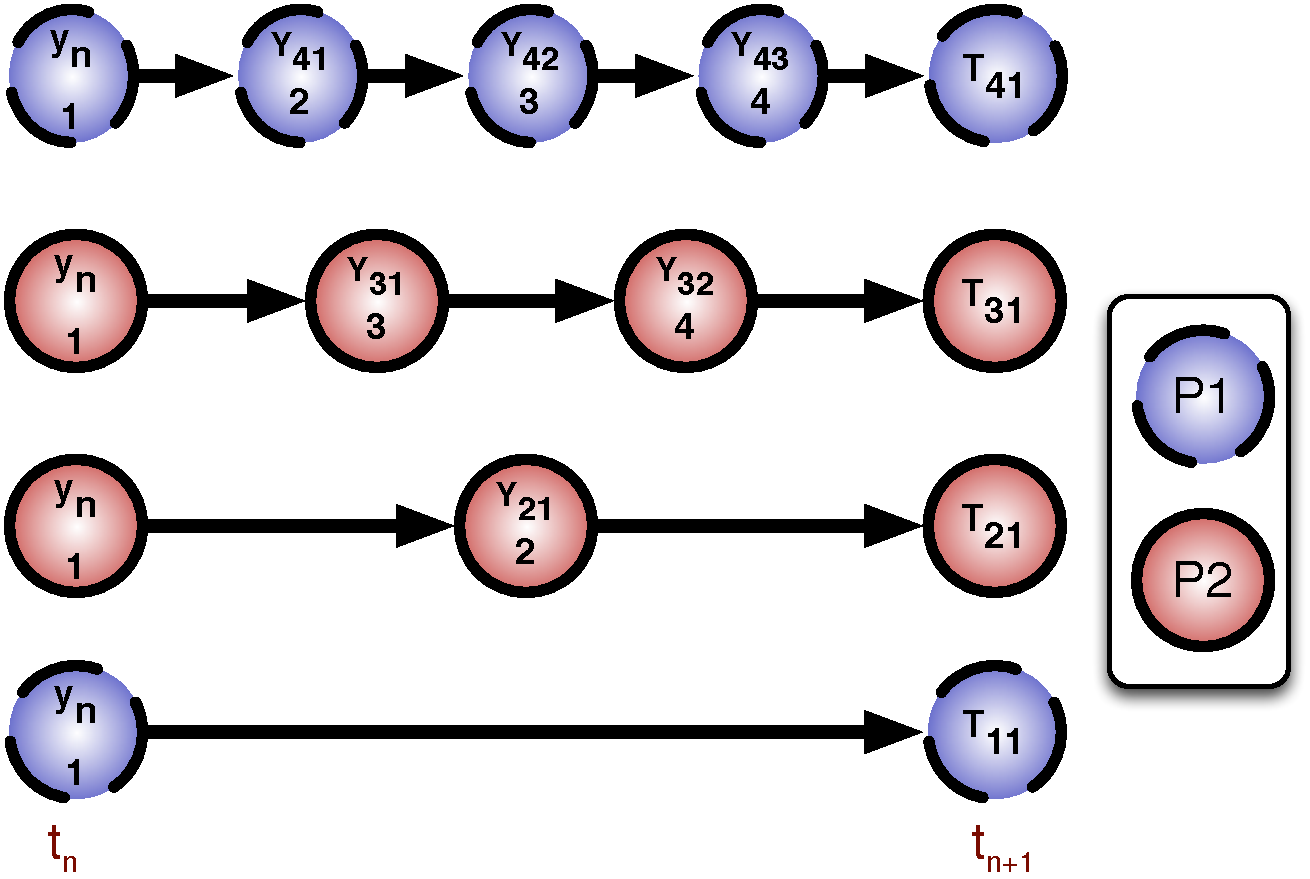
\includegraphics[height=0.4\textwidth]{images/extrap_2proc.pdf}
    \caption {Exploiting concurrency in an Euler extrapolation step using 2 processes.
    The blue circles with broken border are computed by process 1 and the red
    circles with solid border are computed by process 2.  Observe that only $\spar=4$
    sequential function evaluations are required for each process, as opposed to
    the $s=7$ sequential evaluations required in serial.
    \label{fig:extrap_2proc}}
    \end{center}
    \end{figure}

Later we will see that other step number sequences can be advantageous,
particularly when dense output is required.  In general the load balancing
problem obtained is a bin packing problem;
in general this problem is NP-hard, but in practice we deal with small cases
and the problem can be solved easily.  
Load balancing for extrapolation has been discussed in \cite{VanderHouwen1990,Rauber1997}.

For implicit methods, each substep requires an algebraic solve.
For nonlinear problems, this typically involves an outer Newton-type
iteration and an inner iterative linear algebraic solver.
Both of these iterations typically converge faster when the
step size is smaller, so the load balancing problem becomes more
difficult.  We do not investigate this issue further in the present
work.

%That leads to the following load balancing problem for extrapolation:
%given a step number sequence $X$ and a number of processors $n$,
%find a partitioning of the set $X$ into at most $n$ subsets such that
%the maximum sum of the values in any subset is minimized.

\subsection{Order and step size adaptation}
In the extrapolation process, low-order approximants are combined
to produce approximations with successively higher order of accuracy.
In the usual way, the difference between higher- and lower-order
approximants can be used to estimate the error in the less-accurate
value.  This estimate is used to decide whether to accept the step
and what order and step size to use for the next step.

\subsubsection{Serial approach}
A comprehensive strategy for adaptation of order and step size in
extrapolation methods is given in \cite{Hairer1993}.  The objective
is to minimize the overall work per unit advancement in time while
satisfying a local error tolerance.
Higher-order means the tolerance can be satisfied under a larger
step size, but it also means more work per step.  The optimal
choice in this tradeoff depends on the local smoothness of the solution;
the smoother the solution, the higher the optimal order.

In practice, an estimated order $k$ is given at the beginning
of a step.  The error is checked first after $k-1$ extrapolation iterations, 
and then (if necessary) after $k$ and $k+1$.  At each of these iterations,
if the error is small enough the solution is accepted.  If the error
is excessively large, the step is rejected and restarted with a smaller
step size.  If the step is accepted, the step size is adjusted
as is the order (by a maximum of $\pm 1$) based on predictions
of the convergence for the next step.  For details, see 
\cite[pp. 233-235]{Hairer1993}.

\subsubsection{Parallel approach}
In the serial approach, one waits to see the size of the error
after $k-1$ iterations before deciding to do perform iteration $k$.
In a parallel implementation, this makes no sense, since the $k$th
iteration must be performend concurrently with the previous $k-1$.
By the same token, it is not reasonable to perform a $k+1$st
iteration if the error is still too large after $k$ iterations;
it is more efficient to simply restart the step with a smaller
step size.
This means that the step size selection should be somewhat more
conservative in parallel, to reduce the likelihood of failure
after the selected number of iterations.


\subsection{Dense output}
If the interval between required output times is similar to or larger
than the typical solver step size, the solver can simply choose step
sizes such that each output time coincides with the end of a step.
However, some applications require output at very finely-spaced intervals,
so that stopping at each output time would require excessively small steps.
In this case it is common to use what is known as a continuous extension
or {\em dense output} formula.  This allows the solution to be evaluated
to high order accuracy not only at the end of a step, but at any intermediate point.
Dense output for explicit extrapolation methods is discussed in \cite[pp. 237-241]{Hairer1993},
and we follow the strategy outlined there (the same strategy implemented in ODEX).
If the solver detects that dense output is required, it uses the step number sequence
$\{2, 6, 10, 14, 18, 22, \dots\}$ in place of the harmonic sequence, and uses
Hermite interpolation to obtain output at the desired times.  An additional check
on the interpolation error is performed before a step is accepted.


\subsection{Numerical results}
In this section we compare our code to $DOPRI5$ and $DOP853$ integrators from $scipy.integrate.ode$. We ran the comparison test on three problems: N-body problem, Burgers' equation, and Korteweg-de Vries (KdV) equation. 

For each problem, we compared the relative global error in the final solution vs. wall clock time. We measure the relative error using the following: $$\frac{\norm{y - y_{ref}}}{\norm{y_{ref}}},$$ where $y$ and $y_{ref}$ are obtained solution and the reference solution, respectively. The reference solutions used for each problem were computed at tight tolerances. The reference solution for the N-body problem is the same reference solution for ODEX-P in [reference to David's camcos paper. The reference solution for KDV equation and Burgers' equation were computed using \parex with the midpoint method base solver and at tolerances of $1^{-15}$ and  $1^{-10}$, respectively.

The tests were run on a workstation with two 2.66 GHz quad-core Intel Xeon processors. We used the midpoint method as the base solver for \parex with the harmonic step number sequence. We used the midpoint extrapolation for testing as it requires about half as many stages per step to obtain an order p, compared to Euler extrapolation: $$ s = \frac{p^2 + 4}{4}.$$ 
\todo{We should also compare accuracy of dense output.}

\subsubsection{N-body problem}
The N-body problem considers N point masses in an inertial frame of reference and moving under mutual gravitational attraction, which is governed by Newton's law of gravity:
$$F_{ij} = G\frac{m_i m_j}{r_{ij}^2},$$
where $G$ is the gravitational constant ($6.674 \times 10^{-11} N \cdot (m/kg)^2$), $m_i$ and $m_j$ are the masses of the $i^{th}$ and $j^{th}$ point masses, and $r_{ij}$ is the distance between the centers of the $i^{th}$ and $j^{th}$ masses.

We tested with $N = 400$. The initial time was 0, and the final time was set to $T = 0.008$.
\begin{figure}[h]
 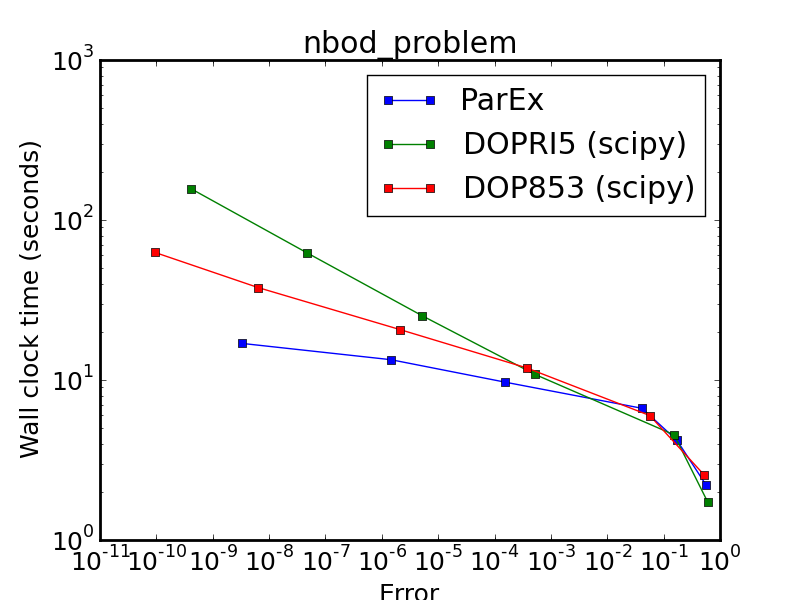
\includegraphics[width=4in]{images/nbod_problem_err_vs_time.png}
\centering
\caption{Runtime versus achieved relative error for N-body problem}
\end{figure} 

\begin{table}
\caption{Speedup for n-body problem\label{tbl:nbody}}{
\begin{tabular}{lcccc}\\
Processes & 1 & 2 & 4 & 6\\ \hline
Run time & 37.49 & 19.80 & 11.36 &  9.81 \\
Average order & 11.79 & 11.79 & 13.99 & 14.27 \\
Ideal speedup &  1.00 &  1.92 &  3.93 &  4.17 \\
Achieved speedup &  1.00 &  1.89 &  3.30 &  3.82 \\
\% of ideal &  1.00 &  0.99 &  0.84 &  0.92 \\ \hline
\end{tabular}}
\end{table}


\subsubsection{KdV equation ($u_t+uu_x+u_{xxx}=0$)}
We solve the equation on $x \in [-\pi,\pi]$  by Fast Fourier transform with the integrating factor $e^{-ik^3t}$ [add reference to Trefethen's "Spectral Methods in MATLAB" book, pages 111-112]

We tested with a a grid size of $N=256$. The initial time and value were $t_0=0$ and $u(0) = 3*25^2/\cosh(0.5*(25*(x+2.)))^2 + 3*16^2/\cosh(0.5*(16*(x+1)))^2 $. The final time was set to $T = 0.003$.
\begin{figure}[h]
 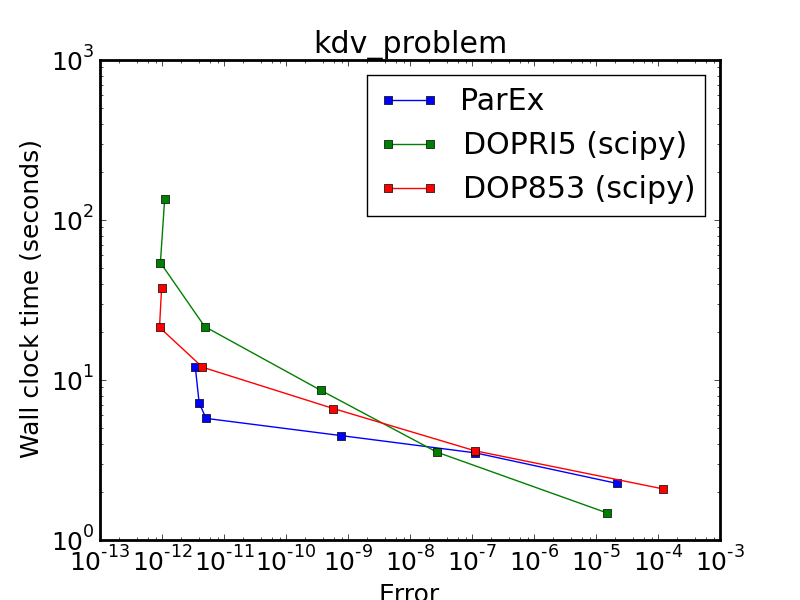
\includegraphics[scale=0.5]{images/kdv_problem_err_vs_time.png}
\centering
\caption{Runtime versus achieved relative error for KdV equation}
\end{figure}

\begin{table}
\caption{Speedup for KdV problem\label{tbl:KdV}}{
\begin{tabular}{lcccc}\\
Processes & 1 & 2 & 4 & 6\\ \hline
Run time & 21.90 & 13.43 &  8.61 &  6.41 \\
Average order & 13.91 & 13.91 & 15.85 & 17.58 \\
Ideal speedup &  1.00 &  2.00 &  3.99 &  4.93 \\
Achieved speedup &  1.00 &  1.63 &  2.54 &  3.42 \\
\% of ideal &  1.00 &  0.82 &  0.64 &  0.69 \\ \hline
\end{tabular}}
\end{table}


\subsubsection{Burgers' equation ($u_t+uu_x=\epsilon u_{xx}$)}
We solve the equation on $x \in [-\pi,\pi]$ by Fast Fourier transform with the integrating factor $e^{\xi^2 \epsilon t}$ [add reference to Trefethen's "Spectral Methods in MATLAB" book, pages 113, exercise 10.6]

We tested with $\epsilon = 0.1$ and a grid size of $N=64$. The initial time and value were $t_0=0$ and $u(0) = \sin^2(x)$ for $x \in [-\pi,0]$ and $0$ otherwise. The final time was set to $T = 3$.
\begin{figure}[h]
 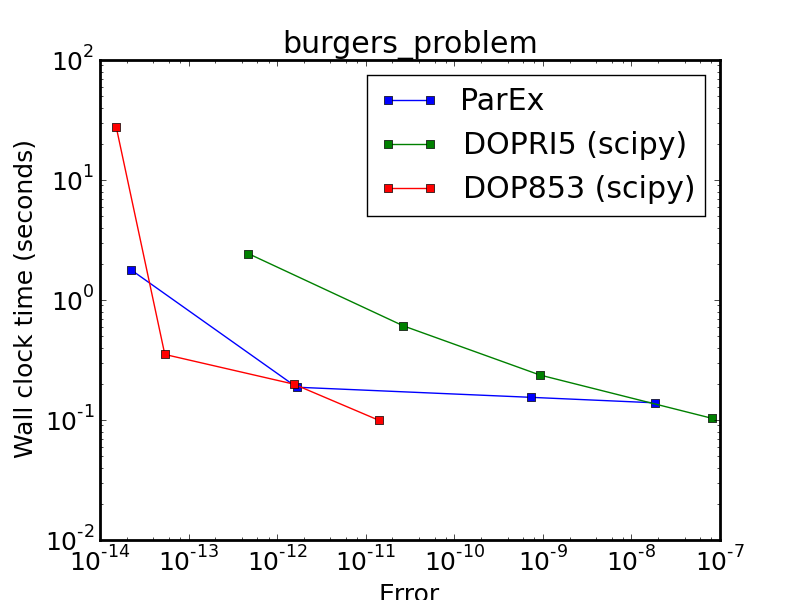
\includegraphics[scale=0.5]{images/burgers_problem_err_vs_time.png}
\centering
\caption{Runtime versus achieved relative error for Burgers' equation}
\end{figure}


\begin{table}
\caption{Speedup for Burgers problem\label{tbl:Burgers}}{
\begin{tabular}{lcccc}\\
Processes & 1 & 2 & 4 & 6\\ \hline
Run time &  3.26 &  2.32 &  1.74 &  1.71 \\
Average order &  7.70 &  7.70 &  8.15 &  8.19 \\
Ideal speedup &  1.00 &  1.97 &  2.67 &  2.70 \\
Achieved speedup &  1.00 &  1.41 &  1.88 &  1.91 \\
\% of ideal &  1.00 &  0.71 &  0.70 &  0.71 \\ \hline
\end{tabular}}
\end{table}


\section{Implicit algorithms}
In this section the extrapolation method will be extended to use implicit step solvers, adequate for stiff problems. In the previous section the efficiency of extrapolation methods with explicit step solvers was proved, nevertheless, these solvers are highly inefficient when solving stiff ODEs.
\begin{itemize}
	\item \underline{Base solver}:  The general extrapolation algorithm for the implicit solver is the same as for the explicit solver with a few differences.\\
    For the implicit solver we use the implicit midpoint rule:
    	$$y_{i+1}=y_{i}+hf((y_{i+1}+y_{i})/2,t_{i}+h/2)$$
    And the implicit Euler method:
    	$$y_{i+1}=y_{i}+hf(y_{i+1},t_{i+1})$$
   Therefore, the main difference between explicit and implicit extrapolation resides in the one step solver.
   
    \item \underline{Order and step size adaptivity}:
   This two characteristics are the same to the explicit extrapolation algorithm. 
   
   Theoretically (add reference book II), this two parameters should consider the additional work performed by the implicit algorithm when evaluating (or estimating) the Jacobian. With this paper's extrapolation implementation, it was observed that this additional work consideration didn't show any performance improvements, so the explicit's algorithm implementation was used (not considering Jacobian calculations). 
    \item \underline{Step number sequence}: In the implicit case, we use the sequence (2,6,10,14,18,...) which is used in the [book II].
    
    After performing a few tests comparing sequences this sequence showed the most promising results.
    
    \item \underline{Semi- vs. fully-implicit}:
    Linearly implicit methods perform a single iteration of the Newton method to find the solution of the implicit step. This way, the iteration cost is reduced by tolerating a coarse implicit step root and allowing the solver to adjust its step for accuracy. The linearly implicit midpoint method (or semi-implicit method) is then:
        $$(I-hJ)(y_{i+1}-y_{i})=-(I+hJ)(y_{i}-y_{i-1})+2hf(y_{i},t_{i})$$

And linearly implicit Euler method:
    	$$(I-hJ)(y_{i+1}-y_{i})=hf(y_{i},t_{i})$$
   
Where $J$ is the Jacobian of $f$ at $(x_{0},y_{0})$ (previous stage final point).

By comparing the performance of both options, it can be seen that  semi-implicit methods are faster than fully-implicit methods.

	\item \underline{Jacobian estimation}:

For the same reason that it is not required an exact solution of the implicit step (thus the use of semi implicit steps), it is not needed an exact estimation of the Jacobian.
Therefore, in our extrapolation algorithm, to estimate the Jacobian, a forward difference formula will be used. This formula has already been used in other ODE solver like LSODE (reference Description and Use of LSODE... pag. 14).

Additionally, as estimating the Jacobian is very expensive (specially for large systems), the Jacobian will be frozen (a new estimation won't be calculated) for different consecutive steps (also done in LSODE solver). Concretely, the Jacobian will be updated (unfrozen) when the step is rejected, as our step was either too large or our Jacobian estimation was not good enough to meet the required error tolerance.

	\item \underline{Smoothing step}:
	The stability domains for the extrapolated midpoint rule (reference II pg 133) show that the A-stability is lost. In order to solve this problem, a smoothing step is performed at the final time for all the extrapolation values (which requires an extra function evaluation
and reduces the order of accuracy by one): 
    $$\hat{T}_{j1} = S_{h_{j}}(x_{0}+H)$$
    $$S_{h}(x) = 1/4(y_{h}(x-h)+2y_{h}(x)+y_{h}(x+h))$$ 
    
Adding this smoothing step improves the performance of the extrapolated midpoint algorithm significantly, by allowing the solver to take bigger integration steps with smaller order. 

For the linearly implicit (semi implicit) midpoint rule, the algorithm described in (reference book II, pg 135), also includes a smoothing step, in this case the step is:
$$S_{h}(x)=1/2(y_{2m-1}+y_{2m+1})$$

For the extrapolated Euler rule and the linearly implicit Euler rule smoothing step is not needed as the algorithms are inherently A-stable (actually, if a smoothing step is added in implicit Euler, the algorithm's performance is worsened).


    \item \underline{Linear solvers}: There are two families of methods that can be used to solve the semi implicit step: exact solvers and iterative methods.
    
    Following the same reasoning used previously, the semi implicit step does not require the machine precision solution an exact solver would provide, instead an approximate solution is enough. For this reason, the best approach, and the most efficient for large systems, is to use an iterative system solver like GMRES.

\end{itemize}


\subsection{Numerical results}

There are four metrics used for the comparison of the solvers:
\begin{itemize}

\item \underline{Time}: execution time.

\item \underline{Function evaluations}: number of calls to the RHS function of the ODE.

\item \underline{Sequential function evaluations}: number of calls to the RHS function that were performed non-simultaneously. This metric shows the improvement of the parallelized code. 

\item \underline{Jacobian evaluations}: number of calls to the analytic Jacobian function.

\end{itemize}

These four metrics are compared against relative global error (same as previous numerical results).

The images shown were calculated with a i7-5500U laptop CPU.

The first result obtained is that among the two semi-implicit methods, Euler semi-implicit has a better performance than Midpoint semi-implicit, specially when requiring stringent tolerances (as expected in [reference book II pg.160]).

\begin{figure}[h]
 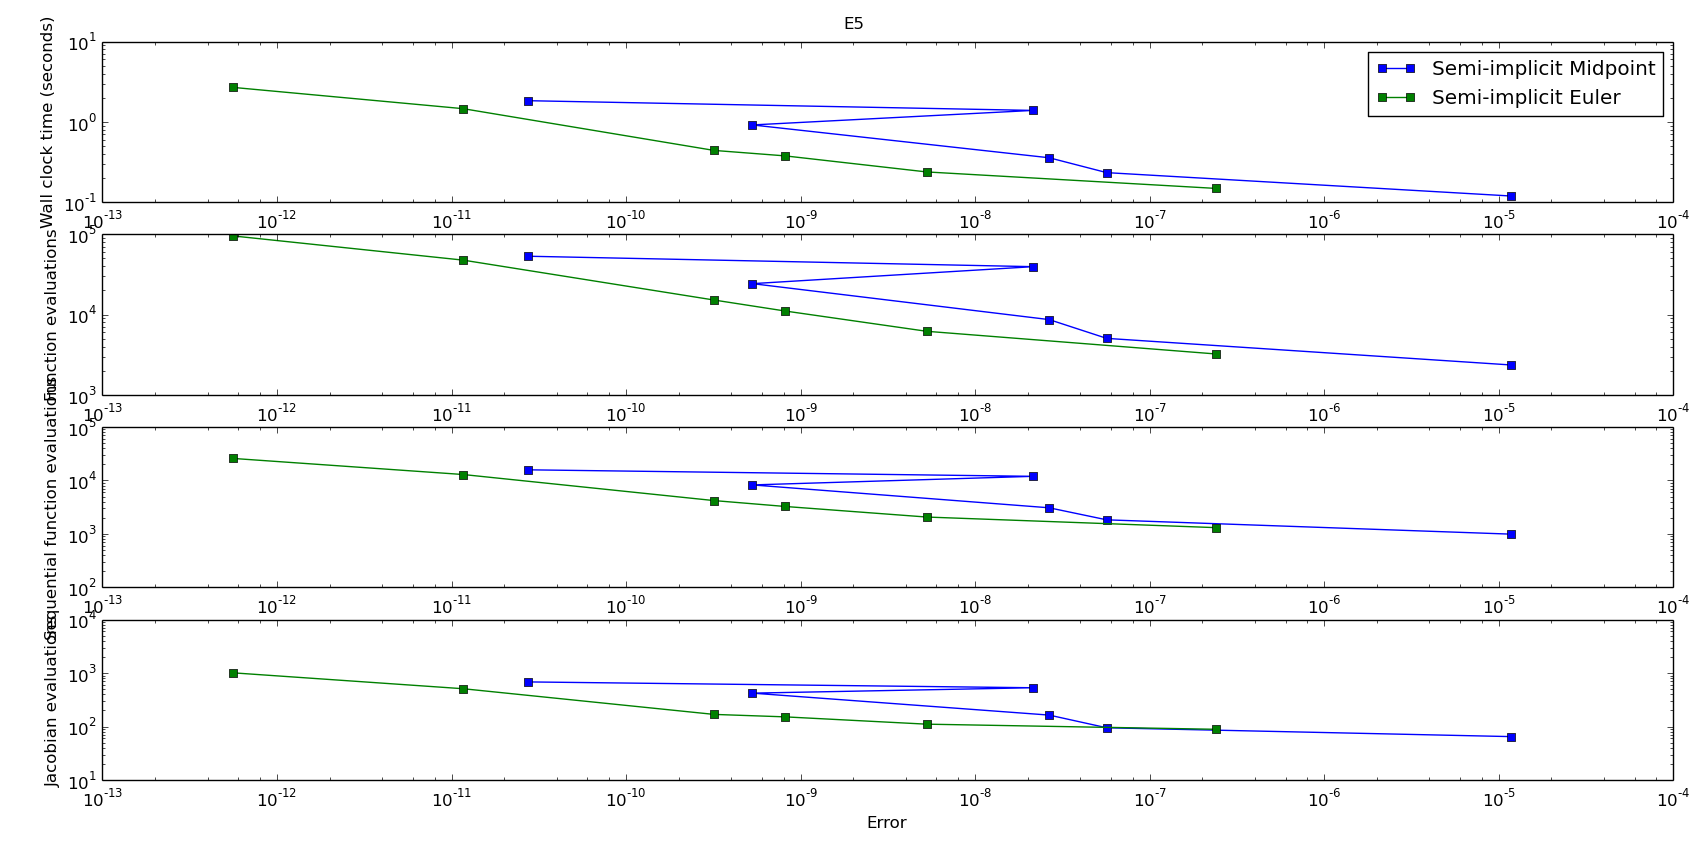
\includegraphics[scale=0.3]{implicit_images/E5_midpoin_euler_g.png}
\centering
\caption{Semi-implicit midpoint and euler comparison of four metrics versus achieved relative error for E5 problem}
\end{figure}

Next, the Euler semi-implicit solver is compared with the python scipy solver odeint [reference to scipy api], which uses lsoda solver form the fortran library odepack.

The comparison is done using these problems.

\subsubsection{VDPOL problem}
The van der Pol problem describes a non-conservative oscillator with a non-linear damping, and it is defined with these equations:

$$y_{1}' = y_{2}$$
$$y_{2}' = ((1-y_{1}^{2})y_{2}-y_{1})/\epsilon, \epsilon=10^{-6}$$
$$y_{1}(0)=2, y_{2}(0)=0; x_{out}=1,2,3,4,...,11$$
VDPOL is a small dimension problem, therefore, the Jacobian is not going to be frozen and an exact linear solver will be used. These are all the results obtained with the VPOL problem:

\begin{figure}[h]
 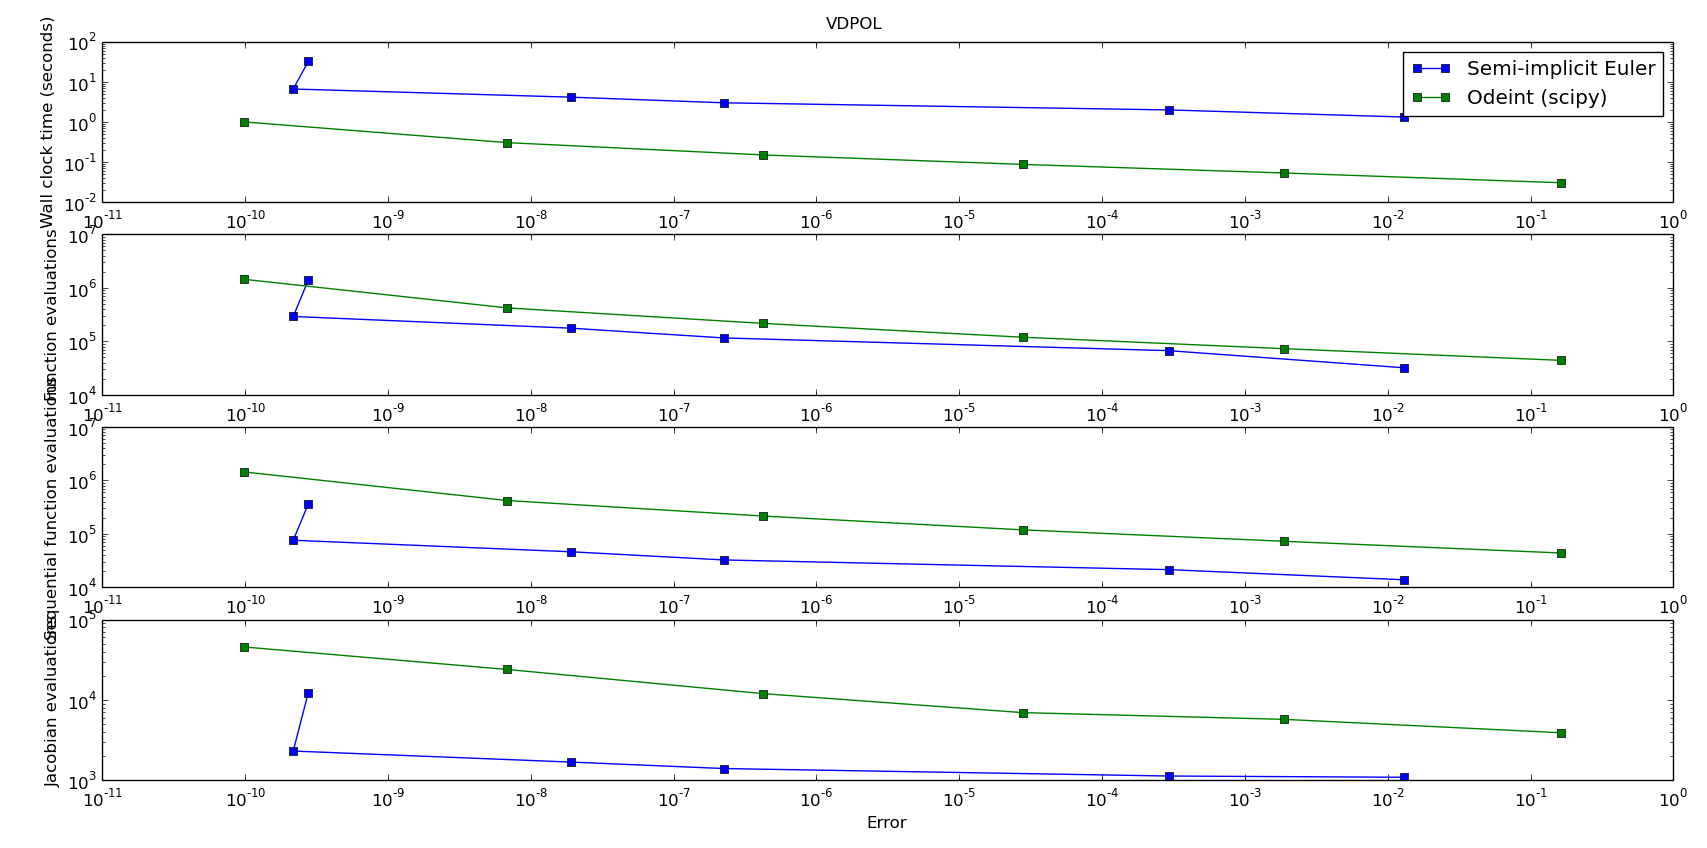
\includegraphics[scale=0.3]{implicit_images/VDPOL_g.png}
\centering
\caption{Semi-implicit euler vs scipy solver comparison for VDPOL problem using an analytic Jacobian}
\end{figure}

\begin{figure}[h]
 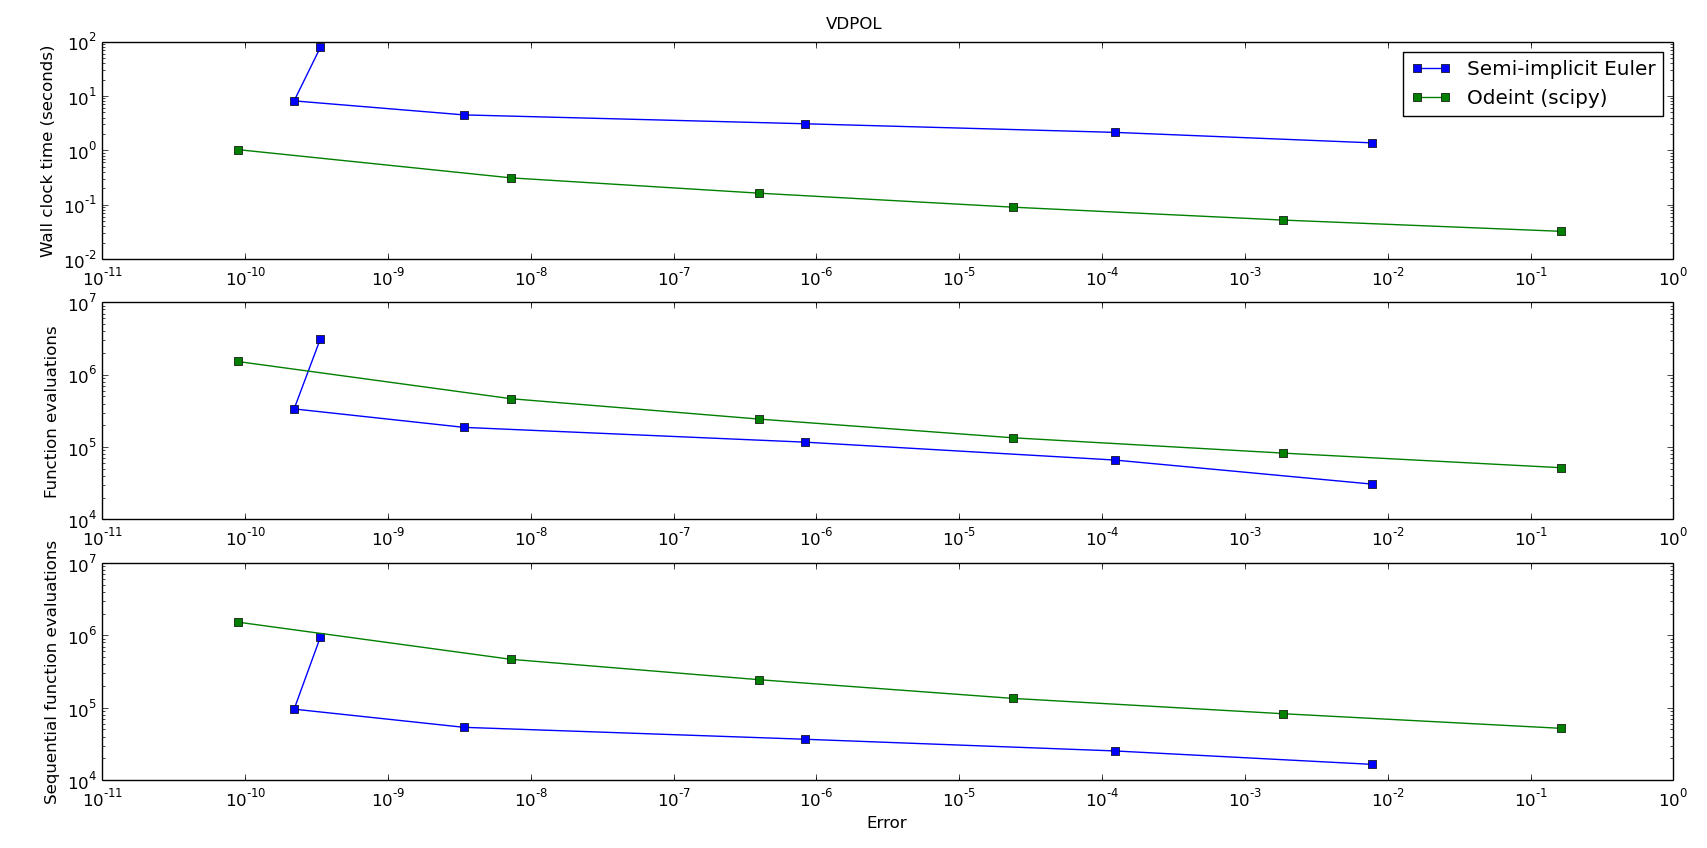
\includegraphics[scale=0.3]{implicit_images/VDPOL_ng.png}
\centering
\caption{Semi-implicit euler vs scipy solver comparison for VDPOL problem estimating the Jacobian}
\end{figure}

\subsubsection{Brusselator problem}
The two-dimensional Brusselator reaction-diffusion problem models an autocatalytic reaction, and it is defined with these equations:
$$\frac{\partial u}{\partial t} = 1+u^{2}v+4.4u+\alpha (\frac{\partial^{2} u}{\partial x^{2}}+\frac{\partial^{2} u}{\partial y^{2}})+f(x,y,t)$$
$$\frac{\partial v}{\partial t} = 3.4u-u^{2}v+\alpha (\frac{\partial^{2} v}{\partial x^{2}}+\frac{\partial^{2} v}{\partial y^{2}})$$
$$where f(x,y,t) = \begin{cases} 5 & \mbox{if } (x-0.3)^{2}+(y-0.6)^2\leq0.1^{2} \mbox{ and } t\geq1.1 \\ 0 & \mbox{else } \end{cases}$$

With initial conditions:

$$u(x,y,0)=22y(1-y)^{3/2}, v(x,y,0)=27x(1-x)^{3/2}$$

Boundary conditions:

$$u(x+1,y,t)=u(x,y,t), u(x,y+1,t)=u(x,y,t)$$

And output points: $x_{out}=1.5$ and $11.5$.

We are going to use a 20x20 ($N=20$) discretization grid of the rectangular diffusion space defined to obtain an ODE system of $2N^{2}=800$ equations.

As this ODE system is much larger, the Jacobian is going to be frozen and the iterative linear solver GMRES will be used.

\begin{figure}[h]
 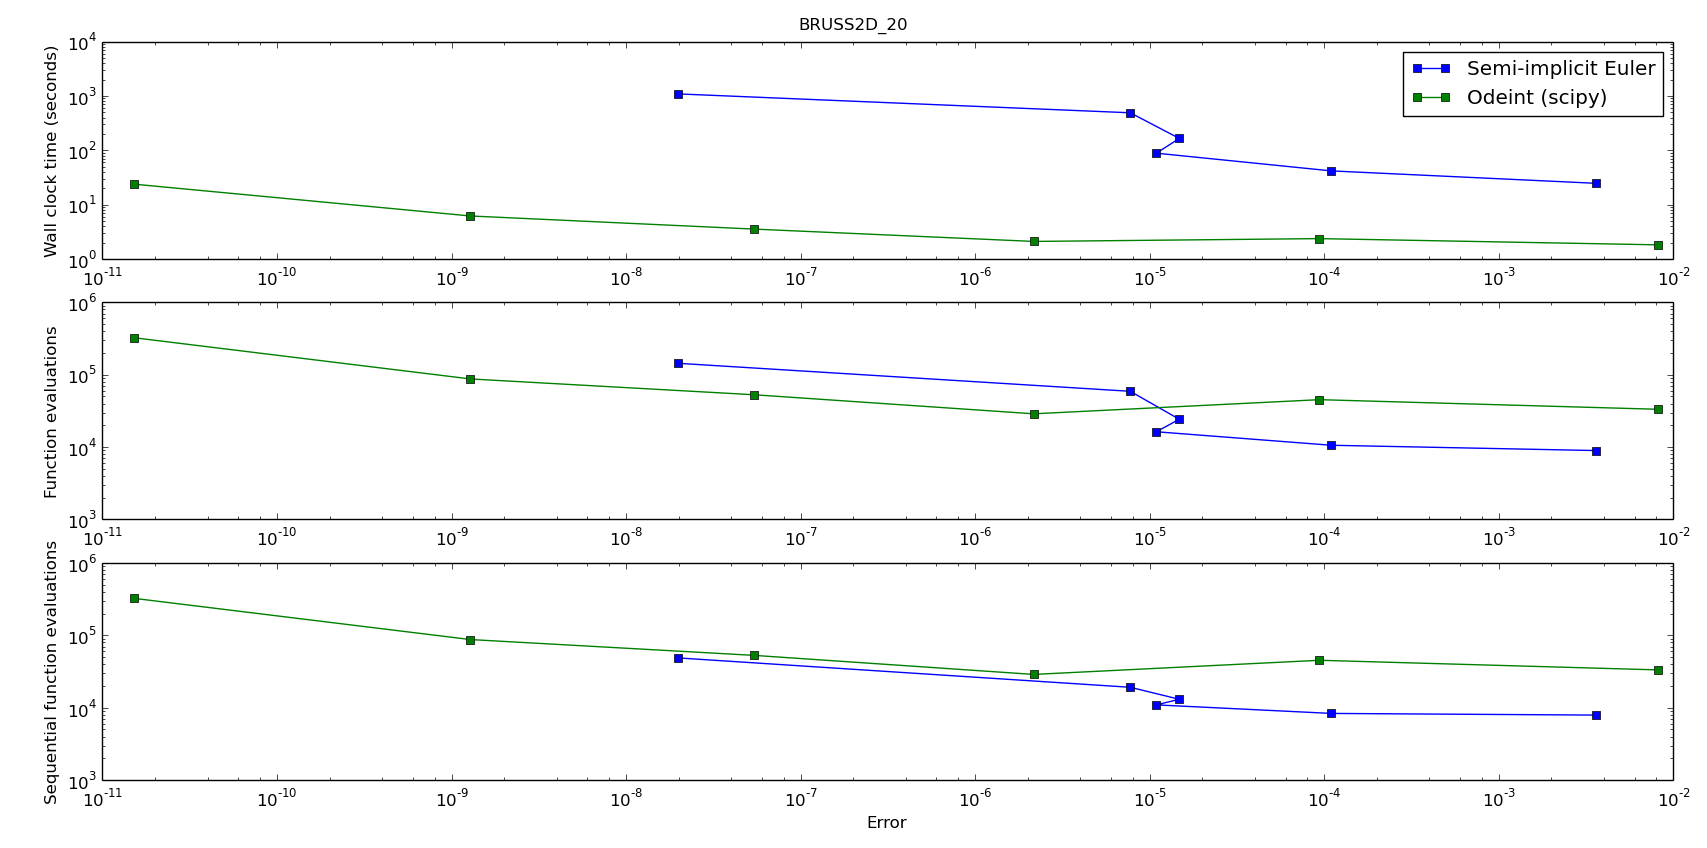
\includegraphics[scale=0.3]{implicit_images/Bruss20_ng.png}
\centering
\caption{Semi-implicit euler vs scipy solver comparison for Brusselator (20x20 grid) problem using an analytic Jacobian}
\end{figure}

\begin{figure}[h]
 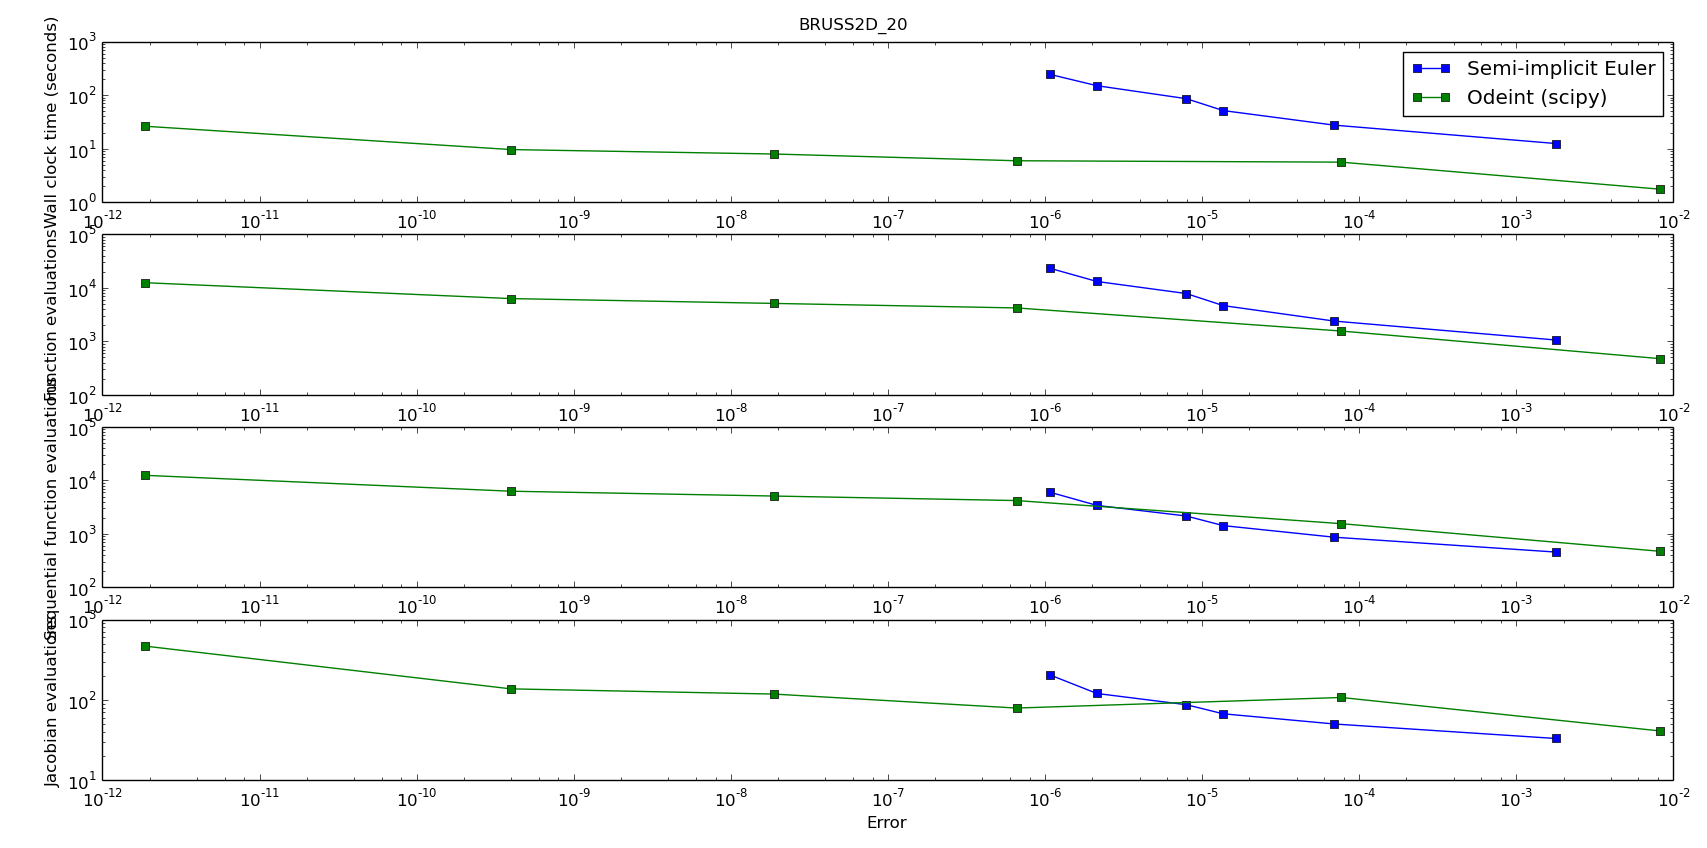
\includegraphics[scale=0.3]{implicit_images/Bruss20_g_fulljac.png}
\centering
\caption{Semi-implicit euler vs scipy solver comparison for Brusselator (20x20 grid) problem estimating the Jacobian}
\end{figure}

If we make use of an analytic sparse Jacobian (which scipy doesn't take advantage of) these results are obtained:

\begin{figure}[h]
 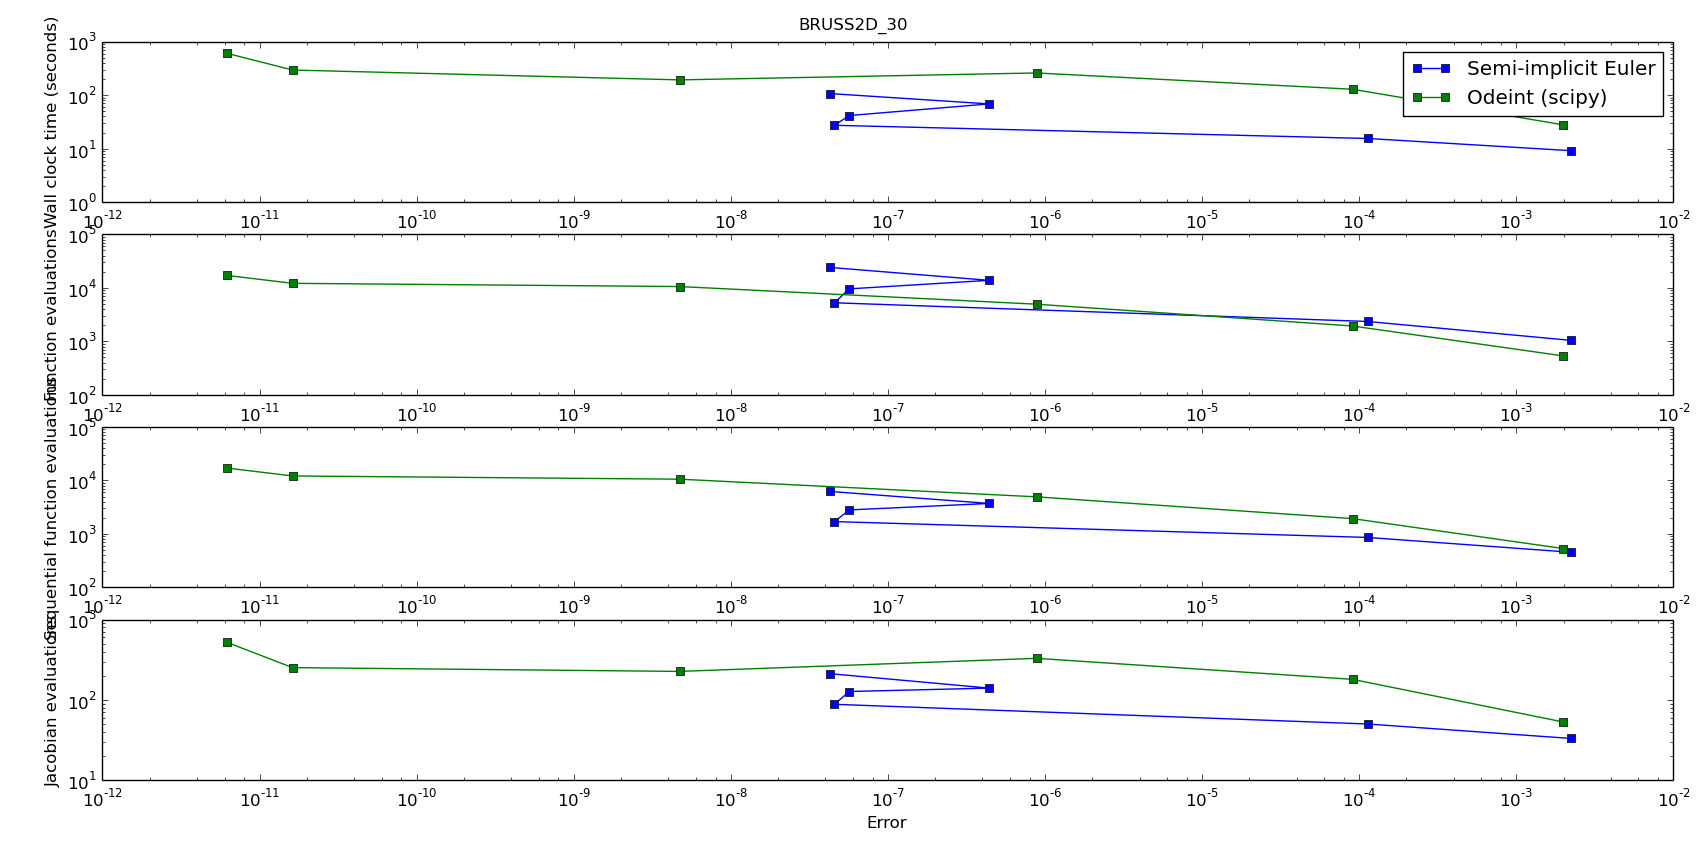
\includegraphics[scale=0.3]{implicit_images/Bruss30_g_sparsejac.png}
\centering
\caption{Semi-implicit euler vs scipy solver comparison for Brusselator (30x30 grid) problem using a sparse analytic Jacobian}
\end{figure}

In this case, because our extrapolation solver operates with the sparse Jacobian, it can outperform the scipy solver, specially when the problem dimension is increased.

\subsubsection{Main obtained results}
\begin{itemize}
\item The time comparison shows that the parallelized implicit extrapolation solver is not faster, except when a sparse analytic Jacobian is used to solve a large problem. 

One of the reasons why it is not faster is that the solver does not parallelize well for large ODE systems. This is because the implicit code uses gmres, which for large systems (where python overhead is negligible) is memory bound (not cpu bound), thus loosing the advantage of using multiple cores.

\item In terms of function evaluations our implicit extrapolation algorithm doesn't, in general, compute less function evaluations. This is as expected, because our solver is not expected to compute less operations sequentially, but to use the straightforward parallelization of such operations.

\item The implicit extrapolation solver outperforms, in most cases, scipy solver when comparing sequential function evaluations. Additionally, when giving the solver an analytic Jacobian, the solver also computes less Jacobian evaluations. Therefore, considering the common assumption that function evaluations are the highest cost operation in ODE solvers, this indicates that for large problems the extrapolation algorithm could outperform other state of the art solvers time-wise.

\end{itemize}

\section{Conclusions}

\subsection{Implicit conclusions}

The implicit extrapolation solver results can be qualified as not definitive, as the solver is still not capable of outperforming in time the current state of the art solvers, but promising. There are four indicators that allow the results to be promising:
\begin{itemize}
\item The explicit algorithm already outperforms in time the state of the art solvers.
\item The sequential function evaluations metric shows that our solver achieves a paralellization, considering the number of function evaluations, that outperforms scipy implicit solver.
\item The current implicit extrapolation algorithm's implementation suffers from a memory bound limitation for large problems, which breaks the CPU parallelization.
\item Python has some overhead over scipy's compiled code implementation. This overhead could become negligible for large problems, but the comparison is then not fair as our solver is then memory-bound.
\end{itemize}

\bibliographystyle{apalike}
\bibliography{main}

\end{document}


